\documentclass[12pt]{article}
\usepackage[a4paper, total={5.5in, 9in}]{geometry}
\usepackage{amsmath}
\usepackage{amsfonts}
\usepackage{graphicx}
\usepackage{pgfplots}
\pgfplotsset{compat=1.18}
\usepackage{enumitem}
\usepackage{hyperref}

\title{College Algebra Worksheet 6.2}
\author{PCL Learning Center}
\date{}

\begin{document}
\maketitle

\section*{Problem Set 1\\Difficulty level: Normal}
\subsection*{Problem 1}
What is the domain and range of the function \(f(x=-3(3)^{x-3}\)?

\subsection*{Problem 2} Graph the function \(f(x)=4^x\) by hand. Plot at least three points on the graph.

\subsection*{Problem 3}
What is the domain and range of the following function?
\[f(x)=\dfrac{7}{2}(2)^{x-1}-5\]

\subsection*{Problem 4}
What is the domain and range of the following function?
\[f(x)=\dfrac{7}{2}(2)^{x+4}+4\]

\subsection*{Problem 5}
Graph the function \(f(x)=-2^{-x}\) by hand. Plot at least three points on the graph.

\subsection*{Problem 6}
The graph of \(f(x)=3x\) is reflected about the \(y\)-axis and stretched vertically by a factor of 4. What is the equation of the new function, \(g(x)\)? State its \(y\)-intercept, domain, and range.

\section*{Problem Set 2\\Difficulty level: Hard}
\subsection*{Problem 1}
The graph of \(f(x)=(1.68)x\) is shifted right 3 units, stretched vertically by a factor of 2, reflected about the \(x\)-axis, and then shifted downward 3 units. What is the equation of the new function, \(g(x)\)? State its \(y\)-intercept (to the nearest thousandth), domain, and range.

\subsection*{Problem 2}
Graph the function \(f(x)=-2(0.25)^{-x}\) by hand. Plot at least three points on the graph.

\newpage
\section*{Solutions to the Set 1}
\subsection*{Problem 1}
domain: \((-\infty,\infty)\)\\
range: \((-\infty,0)\)
\subsection*{Problem 2}
    \begin{center}
    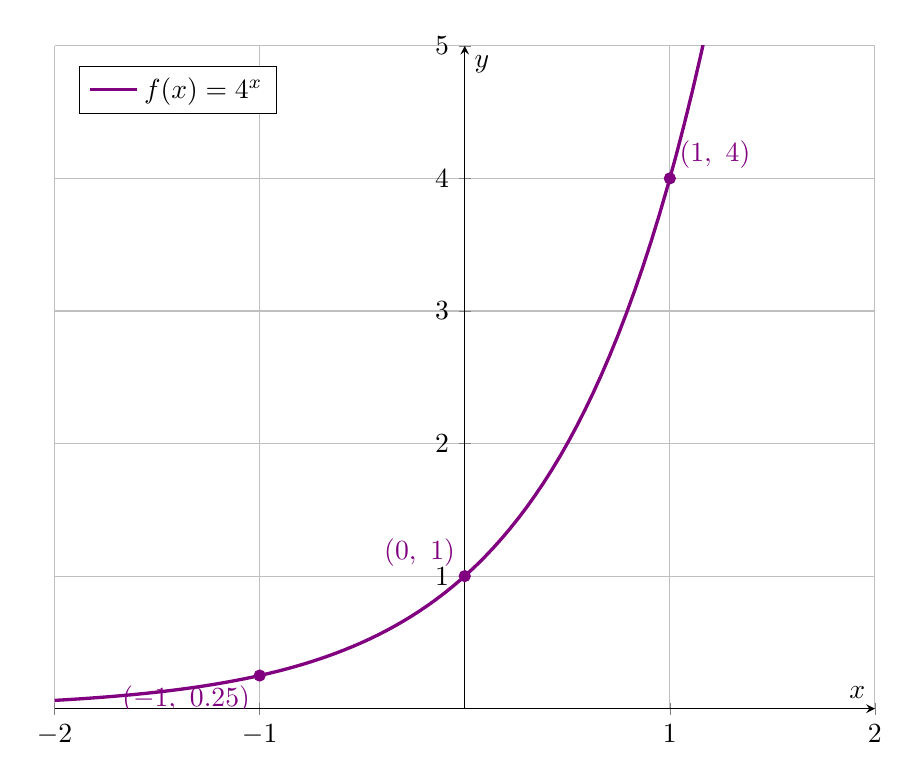
\begin{tikzpicture}
    \begin{axis}[
        axis lines=middle,
        width=12cm,
        height=10cm,
        xmin=-2, xmax=2,
        ymin=0, ymax=5,
        xtick={-2,...,2},
        ytick={0,1,2,3,4,5},
        grid=both,
        xlabel=\(x\),
        ylabel=\(y\),
        legend pos=north west,
        clip=true % Evita que la gráfica y etiquetas salgan del marco
    ]
    \addplot[domain=-2:2, samples=100, very thick, violet] {4^x};
    \addlegendentry{\(f(x) = 4^x\)}
    
    % Puntos específicos y sus etiquetas
    \addplot[only marks, mark=*, violet] coordinates {(-1,0.25) (0,1) (1,4)};
    \node[anchor=north east, violet] at (axis cs:-1,0.25) {\((-1,\ 0.25)\)};
    \node[anchor=south east, violet] at (axis cs:0,1) {\((0,\ 1)\)};
    \node[anchor=south west, violet] at (axis cs:1,4) {\((1,\ 4)\)};
    \end{axis}
    \end{tikzpicture}
    \end{center}
    
\subsection*{Problem 3}
domain: \((-\infty,\infty)\)\\
range: \((-5,\infty)\)
\subsection*{Problem 4}
domain: \((-\infty,\infty)\)\\
range: \((4,\infty)\)
\subsection*{Problem 5}
    \begin{center}
    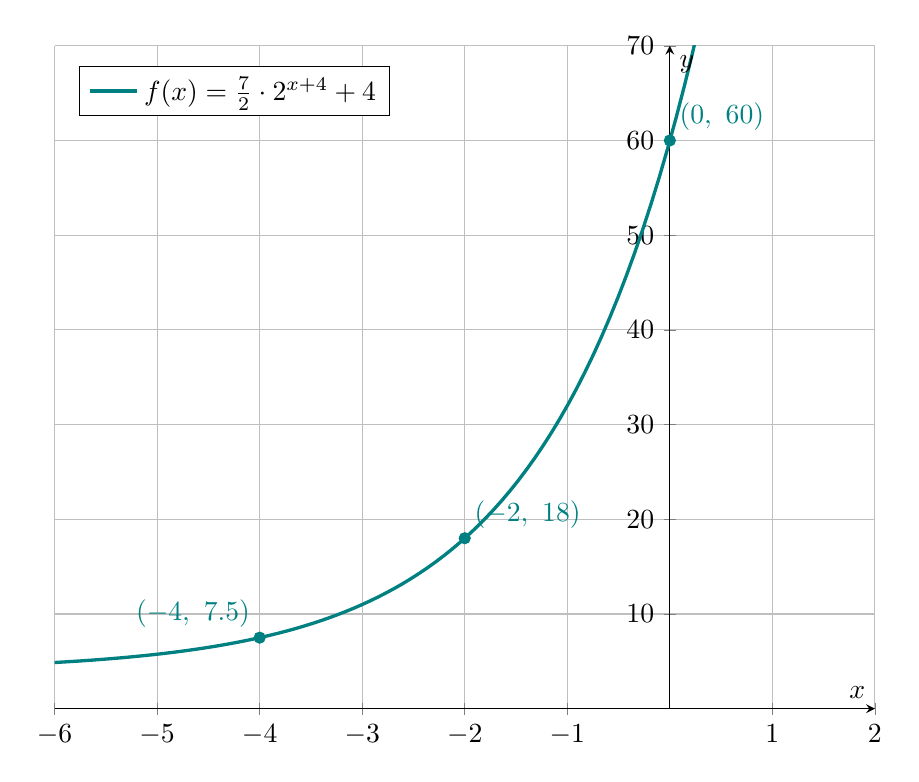
\begin{tikzpicture}
    \begin{axis}[
        axis lines=middle,
        width=12cm,
        height=10cm,
        xmin=-6, xmax=2,
        ymin=0, ymax=70,
        xtick={-6,...,2},
        ytick={0,10,20,30,40,50,60,70},
        grid=both,
        xlabel=\(x\),
        ylabel=\(y\),
        legend pos=north west,
        clip=true
    ]
    \addplot[domain=-6:2, samples=100, very thick, teal] {(7/2)*2^(x+4)+4};
    \addlegendentry{\(f(x) = \frac{7}{2} \cdot 2^{x+4} + 4\)}
    
    % Puntos y etiquetas
    \addplot[only marks, mark=*, teal] coordinates {(-4,7.5) (-2,18) (0,60)};
    \node[anchor=south east, teal] at (axis cs:-4,7.5) {\((-4,\ 7.5)\)};
    \node[anchor=south west, teal] at (axis cs:-2,18) {\((-2,\ 18)\)};
    \node[anchor=south west, teal] at (axis cs:0,60) {\((0,\ 60)\)};
    \end{axis}
    \end{tikzpicture}
    \end{center}

\subsection*{Problem 6}
Original function: \( f(x) = 3x \)\\
Reflection about the \( y \)-axis: \( f(-x) = 3(-x) = -3x \)\\
Vertical stretch by factor of 4: \( g(x) = 4(-3x) = -12x \)\\
\[
\boxed{g(x) = -12x}
\]
\textbf{y-intercept:} \( g(0) = -12(0) = 0 \Rightarrow (0, 0) \)\\
\textbf{Domain:} \( \boxed{(-\infty, \infty)} \)\\
\textbf{Range:} \( \boxed{(-\infty, \infty)} \)\\

\section*{Solutions to the Set 2}
\subsection*{Problem 1}
Original function: \( f(x) = 1.68x \)\\
Shift right by 3: \( f(x - 3) = 1.68(x - 3) \)\\
Vertical stretch by factor of 2: \( 2f(x - 3) = 2 \cdot 1.68(x - 3) \)\\
Reflection over the \(x\)-axis: \( -2f(x - 3) = -2 \cdot 1.68(x - 3) \)\\
Shift down by 3: \( g(x) = -2 \cdot 1.68(x - 3) - 3 \)\\
\[
\boxed{g(x) = -2 \cdot 1.68(x - 3) - 3}
\]
\textbf{y-intercept:} \( g(0) = -2 \cdot 1.68(0 - 3) - 3 = 7.08 \Rightarrow \boxed{(0,\ 7.08)} \)\\
\textbf{Domain:} \( \boxed{(-\infty, \infty)} \)\\
\textbf{Range:} \( \boxed{(-\infty, \infty)} \)\\

\subsection*{Problem 2}
    \begin{center}
    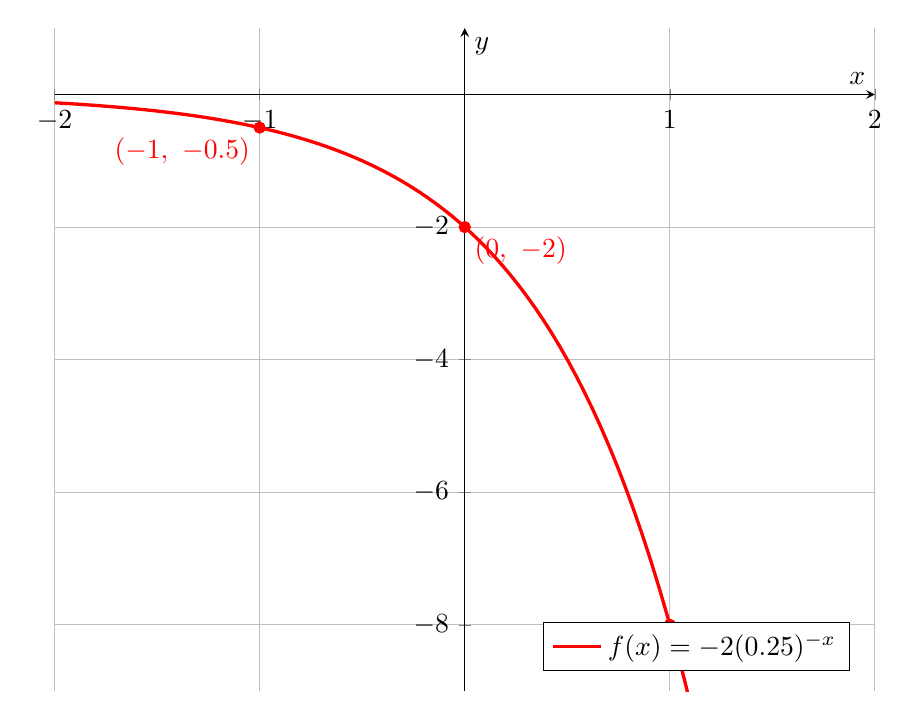
\begin{tikzpicture}
    \begin{axis}[
        axis lines=middle,
        width=12cm,
        height=10cm,
        xmin=-2, xmax=2,
        ymin=-9, ymax=1,
        xtick={-2,...,2},
        ytick={-8,-6,-4,-2,0},
        grid=both,
        xlabel=\(x\),
        ylabel=\(y\),
        legend pos=south east,
        clip=true
    ]
    \addplot[domain=-2:2, samples=100, very thick, red] {-2*(0.25)^(-x)};
    \addlegendentry{\(f(x) = -2(0.25)^{-x}\)}
    
    % Puntos específicos y etiquetas
    \addplot[only marks, mark=*, red] coordinates {(-1,-0.5) (0,-2) (1,-8)};
    \node[anchor=north east, red] at (axis cs:-1,-0.5) {\((-1,\ -0.5)\)};
    \node[anchor=north west, red] at (axis cs:0,-2) {\((0,\ -2)\)};
    \node[anchor=north west, red] at (axis cs:1,-8) {\((1,\ -8)\)};
    \end{axis}
    \end{tikzpicture}
    \end{center}


\end{document}
